\documentclass[a4paper, 12pt]{article}
\usepackage{comment} % enables the use of multi-line comments (\ifx \fi) 
\usepackage{lipsum} %This package just generates Lorem Ipsum filler text. 
\usepackage{fullpage} % changes the margin
\usepackage{indentfirst}
\usepackage{graphicx}
\graphicspath{{./images/}}
\begin{document}
%Header-Make sure you update this information!!!!
\noindent
\large\textbf{Understanding Git} \hfill \textbf{Filippo Cesaratto} \\
\normalsize

\section*{What is git?}
Git is a type of \textbf{version control system} (VCS) that makes it easier to track changes to files. For example, when you edit a file, git can help you determine exactly \emph{what} changed, \emph{who} changed it, and why.

It's useful for coordinating work among multiple people on a project, and for tracking progress over time by saving ``checkpoints''. 

\section*{The three states}
Each file in the \emph{working directory} can be in one of these two states: \emph{tracked} or \emph{untracked}. Tracked files are the files that git knows about. In fact these files had to be present in the last \emph{snapshot} git took, and can have one of these three possible states:
\paragraph{Committed/Unmodified} This means that the data is safely stored in your local database.
\paragraph{Modified} This means that you have changed your file, but have not committed it to your database yet.
\paragraph{Staged} This means that you have marked a modified file in its current version to go into your next commit snapshot.

\vspace*{5mm}
\begin{figure}[h]
	\centering
	\includegraphics{FilesStates}
\end{figure}

\section*{Common commands}
Below is a series of basic commands with descriptions of what they each do.

\paragraph{git help $<$command$>$} This opens the browser and displays information about the given \textbf{command}. If a refresher is all that it's needed, just type: \textbf{git $<$command$>$ -h}.

\paragraph{git init}
This starts your own \emph{repository} from scratch in any existing folder on your computer. Git stores information about changes of the local (in the folder $F$ where git is initialized) files in a data structure called a \emph{repository}. This \emph{repository} is stored in a \emph{.git} directory inside the folder $F$ that is called the \emph{working directory}. No file of the folder $F$ is tracked yet.

\paragraph{git clone $<$URL$>$ [$<$FolderName$>$]}
This downloads an existing repository from the internet to your computer and extract the latest \emph{snapshot}. Almost all the files are downloaded so there is the possibility to open a previous snapshot of the downloaded project. By default it will be saved in the same folder where your repository is in, using the same name as the downloading snapshot, but if the optional parameter \textbf{$<$FolderName$>$} is given, then that would be its name.

\paragraph{git status}
This will print some basic information, such as which files have recently been modified.

\paragraph{git branch $<$newBranchName$>$}
This creates a local checkpoint technically called a \emph{reference} with the given \textbf{newBranchName}. A branch is an active line of development. The most recent commit on a branch is referred as the tip of that branch.

\paragraph{git checkout $<$existingBranchName$>$}


































\end{document}
